\documentclass{beamer}

% Theme
\usetheme{Berlin}
\usecolortheme{default}

% Packages
\usepackage{amsmath, amssymb}
\usepackage{algorithm}
\usepackage{algorithmic}
\usepackage{graphicx}
\usepackage{hyperref}
\usepackage{multirow}


% ----------------------------------------

% Title info
% Added a short title [] for the footer
\title[FedPCL for Recommendation]{Personalized Federated Contrastive Learning\\for Recommendation}
\subtitle{Presentation based on FedPCL paper (2025)}
\author{BTP Group Project}
\institute{IIIT Sri City}
\date{14 February 2026}
\logo{
\includegraphics[height=0.8cm]{iiits-logo-small.png}\hspace*{0.3cm}}


\setbeamertemplate{footline}{
  \leavevmode%

  % -------- First Bar (Author + Page No) --------
  \hbox{%
    \begin{beamercolorbox}[wd=.8\paperwidth,ht=2.6ex,dp=1ex,left]{author in head/foot}%
      \hspace{0.3cm}\insertshortauthor
      \hspace{0.1cm}
      (IIIT Sri City)
    \end{beamercolorbox}%
    \begin{beamercolorbox}[wd=.2\paperwidth,ht=2.5ex,dp=1ex,right]{author in head/foot}%
      \insertframenumber{} / \inserttotalframenumber
      \hspace{0.3cm}
    \end{beamercolorbox}%
  }

  % -------- Second Bar (Paper Title Full Width) --------
  \hbox{%
    \begin{beamercolorbox}[wd=\paperwidth,ht=2.5ex,dp=1ex,left]{title in head/foot}%
      \hspace{0.2cm}
      Personalized Federated Contrastive Learning for Recommendation
    \end{beamercolorbox}%
  }
}


\begin{document}

%------------------------------------------------
% Slide 1
\begin{frame}[plain]

% ----- Blue title box -----
\vspace*{0.5cm}
\begin{beamercolorbox}[wd=\paperwidth,ht=2.6cm,center]{title}
    \usebeamerfont{title}
    Personalized Federated Contrastive Learning\\
    for Recommendation

    \vspace{0.3cm}
    \usebeamerfont{subtitle}
    Presentation based on FedPCL paper
\end{beamercolorbox}

\vspace{0.8cm}

% ----- Black text block -----
\centering
{\large IIIT Sri City --- Group Project \par}
\vspace{0.4cm}

{\normalsize
Anish Mahapatra (S20240020269) \par
Saumya Suman (S20240020330) \par
Mithil Patidar (S20240010143) \par
}

\vspace{0.5cm}

{\normalsize
Under the guidance of \par
\textbf{Dr Rajendra Prasath} \par
}

\vspace{0.6cm}

{\normalsize 17 February 2026}

\end{frame}

%------------------------------------------------
% Slide 2
\begin{frame}{Outline}
\tableofcontents
\end{frame}

%------------------------------------------------
%------------------------------------------------
\section{Introduction}

% Slide 3
\begin{frame}{Introduction}
\small
\begin{itemize}

\item \textbf{Federated Learning (FL):} Enables privacy-preserving recommendation by keeping user data decentralized and sharing only model updates.

\item \textbf{Graph Neural Networks (GNNs):} Model user–item interactions as graphs to capture high-order structural relationships.

\item \textbf{Structural Contrastive Learning:} Enhances node representations by pulling structural neighbors closer in the embedding space.

\item \textbf{FedPCL (Federated Personalized Contrastive Learning):} Combines Federated Learning, Structural Contrastive Learning, and Cluster-based Personalization to learn accurate and user-specific recommendation models.

\end{itemize}

\end{frame}
%------------------------------------------------
% Slide 4
\begin{frame}{Motivation}
\small
\begin{itemize}

  \item \textbf{Privacy Concerns:}  
  Traditional recommendation systems collect user data on a central server,
  which creates privacy and security risks.

  \item \textbf{Federated Learning Challenge:}  
  Federated learning keeps user data on local devices,
  but makes model training more difficult.

  \item \textbf{Data Sparsity:}  
  Each user has only a small amount of data,
  so learning good user and item representations is hard.

  \item \textbf{Non-IID Problem:}  
  Users have different preferences (non-IID data),
  so one global model does not work well for everyone.

\end{itemize}
\end{frame}



%-----------------------------------------------------
% Slide 5
\begin{frame}{Contributions (from the paper)}
  \begin{enumerate}
    \item Propose \textbf{FedPCL}: personalized FL framework that combines structural contrastive learning with multicenter aggregation.
    \item Design \textbf{structure-aware contrastive objective} leveraging GNN layer outputs (structural neighbors).
    \item Propose \textbf{cluster-level + global model aggregation} to form personalized models for each client.
    \item Extensive experiments on five datasets showing consistent performance gains vs baselines.
  \end{enumerate}
\end{frame}

%-----------------------------------------------------
\section{Related Work}
% Slide 6
\begin{frame}{Related Work: GNNs for Recommendation}

\begin{itemize}
  \item User–item interactions naturally form a \textbf{bipartite graph}.
  \item \textbf{Graph Neural Networks (GNNs)} propagate information through neighbors to capture higher-order relationships.
  \item \textbf{LightGCN (He et al., SIGIR 2020)} simplifies GCNs by removing feature transformation and nonlinearities.
  \item GNN-based models significantly outperform MF-based methods in sparse recommendation settings.
\end{itemize}

\end{frame}

% Slide 7
\begin{frame}{Related Work: GNNs for Recommendation (Illustration)}

\centering
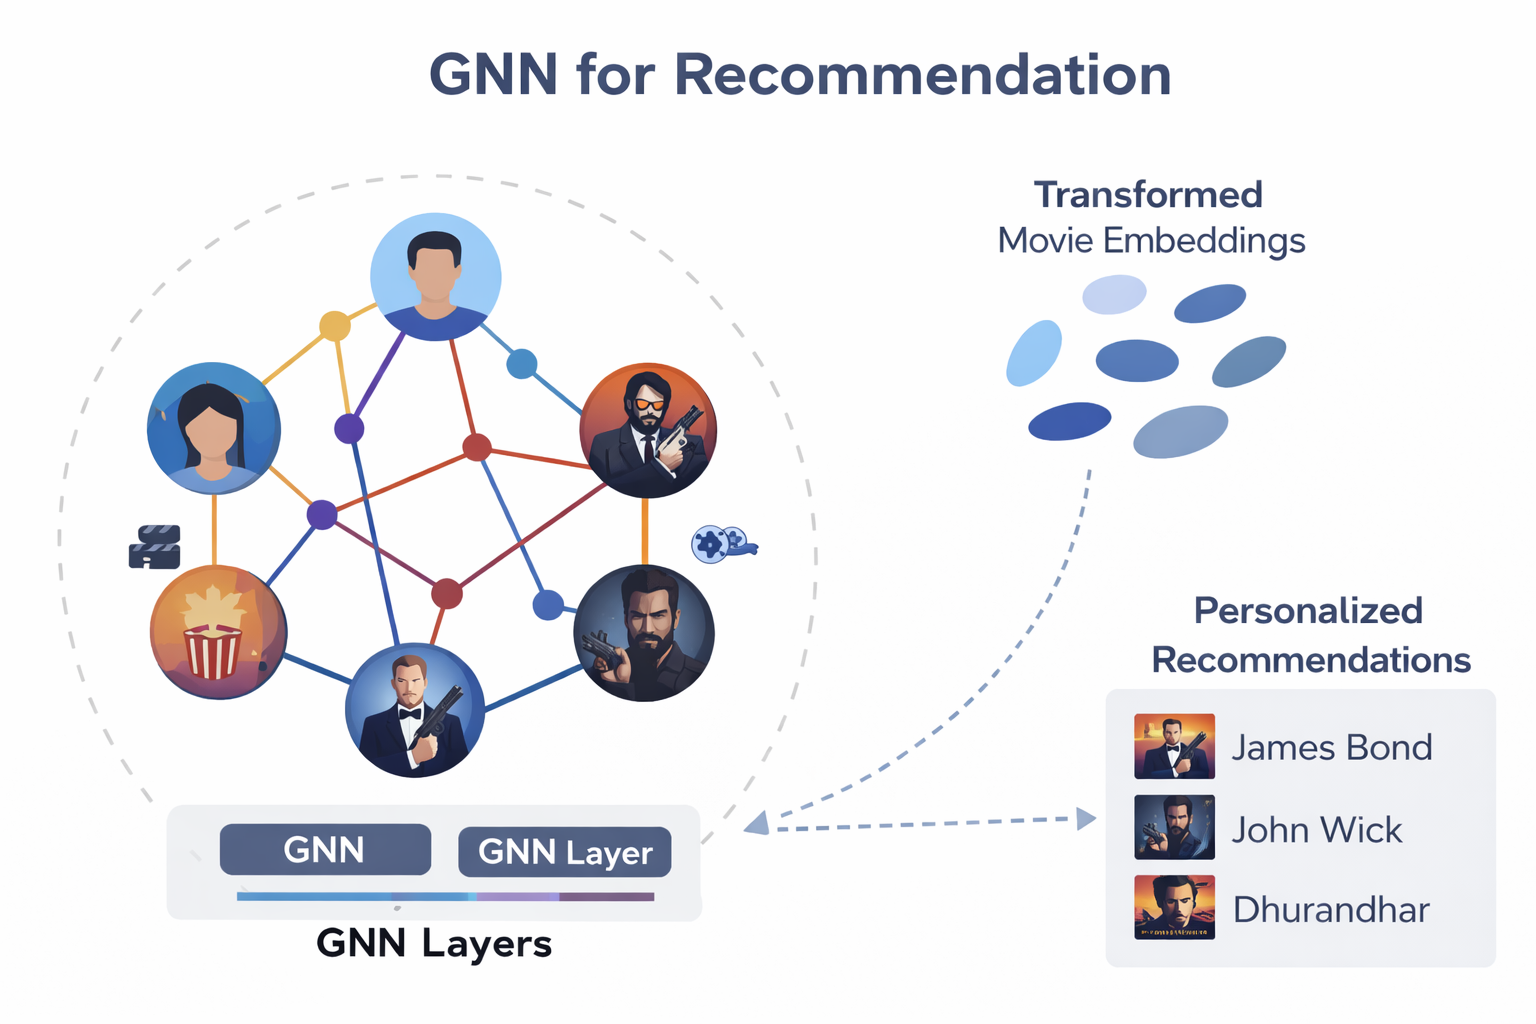
\includegraphics[height=0.80\textheight, keepaspectratio]{gnn_recommendation.png}

\end{frame}


% Slide 8
\begin{frame}{Related Work: Contrastive Learning}

\begin{itemize}
  \item \textbf{Contrastive Learning (CL)} is a self-supervised learning paradigm. Self-supervised learning means the model creates supervision signals from the data itself, without requiring manually labeled data.
  \item It maximizes agreement between \textbf{positive pairs} and minimizes similarity with \textbf{negative pairs} using \textbf{InfoNCE loss}.
  \item CL is self-supervised because it constructs positive and negative pairs directly from the input data (e.g., different views or structural neighbors), instead of using external labels.
\end{itemize}

\end{frame}

% Slide 9
\begin{frame}{Related Work: Contrastive Learning (Illustration)}

\centering
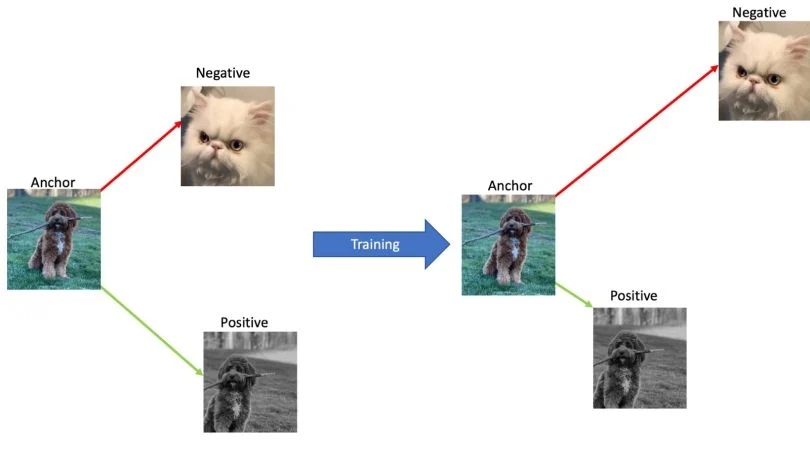
\includegraphics[height=0.7\textheight, keepaspectratio]{contrastive_learning_graph.png}

\end{frame}


% Slide 10
\begin{frame}{Related Work: Federated Recommendation}

\begin{itemize}
  \item \textbf{Federated Learning (FL)} enables collaborative training without sharing raw user data.
  \item \textbf{FedAvg (McMahan et al., 2017)} aggregates local models but assumes IID data.
  \item Extensions such as \textbf{FedMF}, \textbf{FedGNN}, and \textbf{PerFedRec (2022)} introduce privacy and personalization.
  \item Key challenges remain: \textbf{non-IID data} and \textbf{data sparsity}.
  \item \textbf{FedPCL} jointly addresses these via GNNs, contrastive learning, and personalized aggregation.
\end{itemize}

\end{frame}

% Slide 11
\begin{frame}{Related Work: Federated Recommendation (Illustration)}

\centering
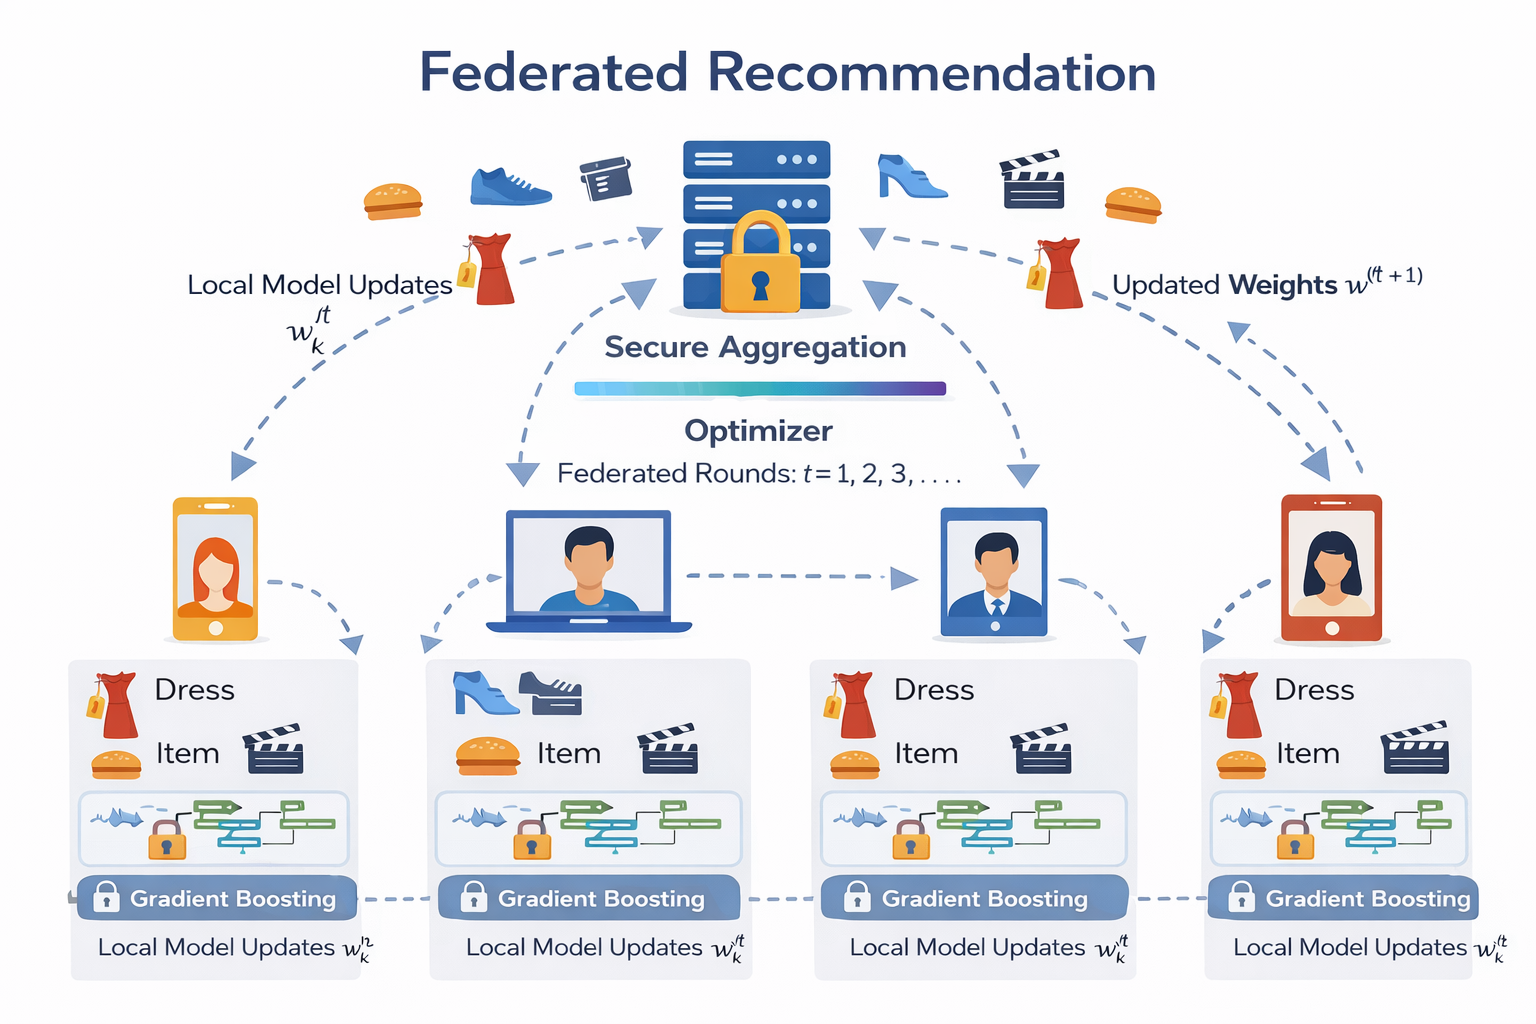
\includegraphics[height=0.8\textheight, keepaspectratio]{federated_recommendation.png}

\end{frame}


%------------------------------------------------
\section{Framework}

% Slide 12
\begin{frame}{Framework Overview}

\textbf{Client side}
\begin{itemize}
  \item Local GNN on user–item subgraph
  \item Structural contrastive loss using even-layer embeddings
  \item BPR(Bayesian Personalized Ranking) ranking loss
  \item Local Differential Privacy (LDP) on gradients
\end{itemize}

\textbf{Server side}
\begin{itemize}
  \item K-means clustering on users
  \item Cluster-level and global aggregation
  \item Personalized model via weighted combination
\end{itemize}

\vspace{0.3cm}
\textbf{Prediction Phase}
\begin{itemize}
  \item Final user embedding $e_u$ and item embedding $e_i$
  \item Predicted preference score:
  \[
  r_{ui} = e_u^\top e_i
  \]
\end{itemize}

\end{frame}

%------------------------------------------------
% Slide 13
\begin{frame}{FedPCL Model Framework}

\centering

\begin{figure}
  \centering
  \begin{minipage}{0.62\textwidth}
    \centering
    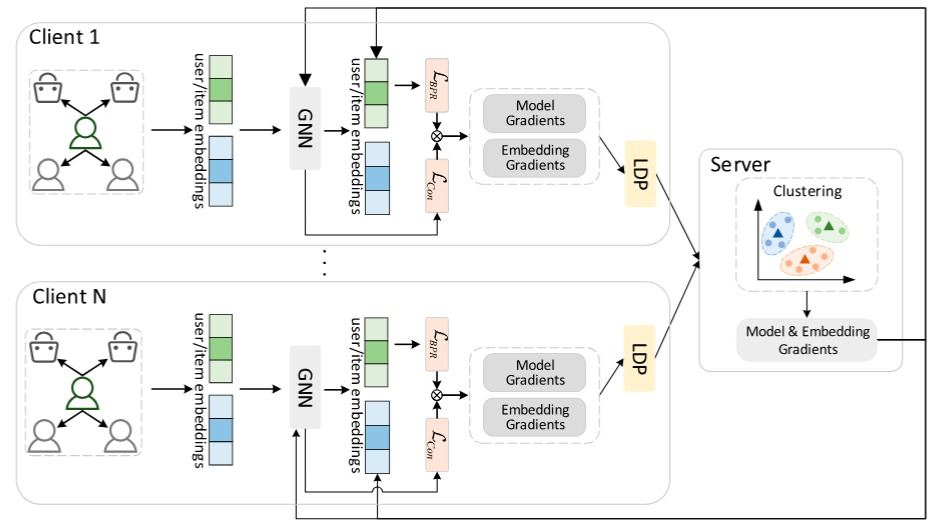
\includegraphics[width=\linewidth]{FedPCL_framework.png}
  \end{minipage}
  \hfill
  \begin{minipage}{0.35\textwidth}
    \centering
    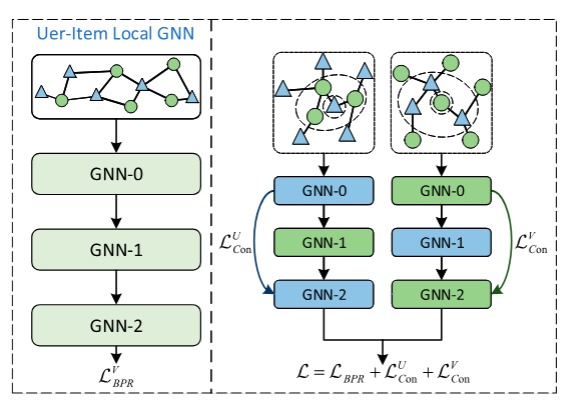
\includegraphics[width=\linewidth]{structure_contrastive_learning.png}
  \end{minipage}
\end{figure}
FedPCL framework (2025) {\color{blue}\hyperlink{ref:fedpcl}{\textit{[7]}}}
\end{frame}



%-----------------------------------------------------
% Slide 15 (New)
\begin{frame}{BPR and Influence of Evidence}
\small

\textbf{What is BPR?}

\begin{itemize}
    \item Bayesian Personalized Ranking (BPR) is a pairwise ranking loss.
    \item Based on observed implicit feedback (user interactions).
\end{itemize}

\textbf{Influence of Evidence:}

\begin{itemize}
    \item Positive interaction $(u,i)$ provides evidence that $i$ is preferred.
    \item Non-interacted item $j$ treated as negative sample.
    \item Strength of evidence depends on interaction frequency.
    \item Sparse data → weaker ranking signal.
\end{itemize}

\textbf{Limitation:}
\begin{itemize}
    \item BPR uses only interaction evidence.
    \item Does not exploit structural similarity.
\end{itemize}

\end{frame}



%-----------------------------------------------------
\section{Key Equations}
% Slide 14
\begin{frame}{Key equations (I)}
\small
  \begin{block}{BPR(Bayesian Personalized Ranking) ranking loss}
    \[
      \mathcal{L}_{\text{BPR}} = - \sum_{(u,i,j)\in \mathcal{D}} \ln \sigma(\hat r_{ui} - \hat r_{uj})
    \]
    where $\hat r_{ui}=f(e_u,e_i)$ (dot-product used in experiments).
  \end{block}
  \begin{block}{Structure-contrastive (InfoNCE) — users}
    \[
    \mathcal{L}_{\text{Con}}^{U} = -\sum_{i\in U}\log \frac{\exp\big(e_i^{(l)}\cdot e_i^{(0)}/\tau\big)}
    {\sum_{j\in U}\exp\big(e_i^{(l)}\cdot e_j^{(0)}/\tau\big)}
    \]
    where $e^{(l)}$ is the GNN output at even layer $l$ (structural neighbor embedding), $e^{(0)}$ initial embedding.
  \end{block}
\end{frame}

% Slide 15
\begin{frame}{Key equations (II)}
\small
\hypertarget{eq:eqn}{}
  \begin{block}{Items contrastive loss (analogous)}
    \[
    \mathcal{L}_{\text{Con}}^{V} = -\sum_{v\in V}\log \frac{\exp\big(e_v^{(l)}\cdot e_v^{(0)}/\tau\big)}
    {\sum_{n\in V}\exp\big(e_v^{(l)}\cdot e_n^{(0)}/\tau\big)}
    \]
  \end{block}
  \begin{block}{Full client loss}
    \[
      \mathcal{L} = \mathcal{L}_{\text{BPR}} + \beta_1\big(\mathcal{L}_{\text{Con}}^{U} + \lambda \,\mathcal{L}_{\text{Con}}^{V}\big) + \beta_2\|\Theta\|_2^2
    \]
  \end{block}
  \begin{block}{Personalized model composition}
    \[
      h_u^{(t)} = \mu_1 h_{C(u)}^{(t)} + \mu_2 h_{\text{global}}^{(t)}
    \]
  \end{block}
\end{frame}



%-----------------------------------------------------
% Slide 16
\begin{frame}{LDP and aggregation}
\small
  \begin{itemize}
    \item \textbf{Local Differential Privacy (LDP)} applied to gradients:
      \hypertarget{eq:ldp}{}
      \[
        \tilde g_u = \mathrm{clip}(g_u,\sigma) + \mathrm{Laplace}(0,\lambda)
      \]
    \item \textbf{Embedding aggregation} (items):
      \[
        \bar g_i = \frac{\sum_{u\in \mathcal{N}_t} m_u \,\tilde g_{u,i}}{\sum_{u\in \mathcal{N}_t} m_u}
      \]
      update: $e_i^{t}=e_i^{t-1}-\eta \bar g_i$.
    \item \textbf{Network aggregation:}
      \[
        \bar g_{C(u)} = \frac{\sum_{u\in C(u)} m_u\,\tilde g_u}{\sum_{u\in C(u)} m_u},\quad
        h_{C(u)} = h_{C(u)} - \eta \bar g_{C(u)}
      \]
      global: average cluster models $h_{\text{global}} = \frac{1}{K}\sum_{k=1}^K h_{C_k}$.
  \end{itemize}
\end{frame}

%-----------------------------------------------------
\section{Algorithm}
% Slide 17


\begin{frame}[fragile]{Algorithm: FedPCL}

\resizebox{!}{0.41\textheight}{
\begin{minipage}{\textwidth}
\begin{algorithm}[H]
\caption{FedPCL}
\begin{algorithmic}[1]

\REQUIRE Embedding size $d$; Learning rate $\eta$; Clients local graph $\{G_n\}_{n=1}^{N}$; 
Initialize $U=[e_n]_{n=1}^{N}$, $V=[e_i]_{i=1}^{M}$, $h_{\text{global}}$

\ENSURE Local client embeddings $U=[e_n]_{n=1}^{N}$; Model parameters $h$

\STATE \textbf{// server}
\WHILE{not converge}
    \STATE Cluster all users $U$ into $K$ clusters \hfill $\triangleright$ user clustering
    \STATE Randomly select a subset $\mathcal{N}$ from user set $U$
    \FOR{each $n \in \mathcal{N}$}
        \STATE $\tilde{g}_i^n, \tilde{g}_{C(n)} \leftarrow \textbf{ClientUpdate}(n, e_i^t, h_C, h_{\text{global}})$
    \ENDFOR
    \STATE $g_i \leftarrow$ Eq.\,{\color{blue}\hyperlink{eq:ldp}{(1)}} \hfill $\triangleright$ item gradients
    \STATE $e_i^t \leftarrow$ Eq.\,{\color{blue}\hyperlink{eq:ldp}{(2)}} \hfill $\triangleright$ item embeddings
    \STATE $h_C^t \leftarrow$ Eq.\,{\color{blue}\hyperlink{eq:eqn}{(3)}} \hfill $\triangleright$ clustering model
    \STATE $h_{\text{global}}^t \leftarrow$ Eq.\,{\color{blue}\hyperlink{eq:eqn}{(4)}} \hfill $\triangleright$ global model
\ENDWHILE

\end{algorithmic}
\end{algorithm}
\end{minipage}
}

\end{frame}


%-----------------------------------------------------
% Slide 18

\begin{frame}[fragile]{Algorithm: FedPCL (Cont.)}

\small

\begin{algorithm}[H]
\begin{algorithmic}[13]

\STATE \textbf{// client}
\STATE \textbf{function} \textsc{ClientUpdate}$(n, e_i^t, h_C, h_{\text{global}})$
    \STATE Calculate the embedding gradients $\nabla U_n$ and $g_i^n$ by {\color{blue}\hyperlink{eq:ldp}{(5)}}
    \STATE Calculate the model gradients $g_m^n$ by Eq.\,{\color{blue}\hyperlink{eq:ldp}{(6)}}
    \STATE $e_n \leftarrow e_n - \eta \nabla U_n$ \hfill $\triangleright$ user embedding
    \STATE $\tilde{g}_i^n, \tilde{g}_{C(n)} \leftarrow$ Eq.\,{\color{blue}\hyperlink{eq:ldp}{(7)}} \hfill $\triangleright$ LDP
    \STATE \textbf{return} $\tilde{g}_i^n, \tilde{g}_{C(n)}$
\STATE \textbf{end function}

\end{algorithmic}
\end{algorithm}

\end{frame}

%-----------------------------------------------------
% Slide-19
\begin{frame}{Computational Complexity Analysis}
\small

% -------- TABLE (FULL WIDTH) --------
\begin{table}
\centering
\begin{tabular}{|c|l|l|}
\hline
\textbf{Side} & \textbf{Component} & \textbf{Time Complexity} \\
\hline

\multirow{3}{*}{Client}
 & GNN Propagation & $\mathcal{O}(L |E| d)$ \\
 & BPR Loss & $\mathcal{O}(|D| d)$ \\
 & Contrastive Loss & $\mathcal{O}(|U|^2 d)$ \\
\hline

\multirow{2}{*}{Server}
 & K-means Clustering & $\mathcal{O}(K N d)$ \\
 & Model Aggregation & $\mathcal{O}(N d)$ \\
\hline

\end{tabular}
\end{table}

\vspace{0.001cm}

% -------- BOTTOM SPLIT --------
\begin{columns}

% ----- LEFT COLUMN -----
\begin{column}{0.5\textwidth}

\textbf{Overall Per Round:}
\[
\mathcal{O}(L|E|d + |D|d + KNd)
\]

\vspace{0.1cm}

\textbf{Communication Cost:}
\[
\mathcal{O}(Nd)
\]

\end{column}

% ----- RIGHT COLUMN -----
\begin{column}{0.5\textwidth}

{\scriptsize
\begin{itemize}
    \item $L$ : number of GNN layers
    \item $|E|$ : number of graph edges
    \item $|D|$ : number of training triplets
    \item $|U|$ : number of users (batch size)
    \item $K$ : number of clusters
    \item $N$ : number of clients
    \item $d$ : embedding dimension
\end{itemize}
}

\end{column}

\end{columns}

\end{frame}





%-----------------------------------------------------
% Slide 19
\begin{frame}{Team Contributions}

\begin{itemize}
  \item \textbf{Anish Mahapatra} -- Worked on the MovieLens-100K dataset, 
  including preprocessing, graph construction, and analysis of sparsity.

  \item \textbf{Mithil Patidar} -- Worked on the FilmTrust dataset, 
  handling data preparation and studying trust-based interaction patterns.

  \item \textbf{Saumya Suman} -- Worked on the Steam-200K dataset, 
  focusing on interaction processing and dataset statistics evaluation.

  \item \textbf{All members} -- Literature review, mathematical formulation, and report preparation.
\end{itemize}

\end{frame}


%-----------------------------------------------------
%================================================
\section{Datasets}

%================================================
%------------------------------------------------
% Slide 20
% MovieLens-100K — Slide 1 (Graph + Text)

\begin{frame}{MovieLens-100K Dataset (Analyzed by Anish Mahapatra)}

\centering
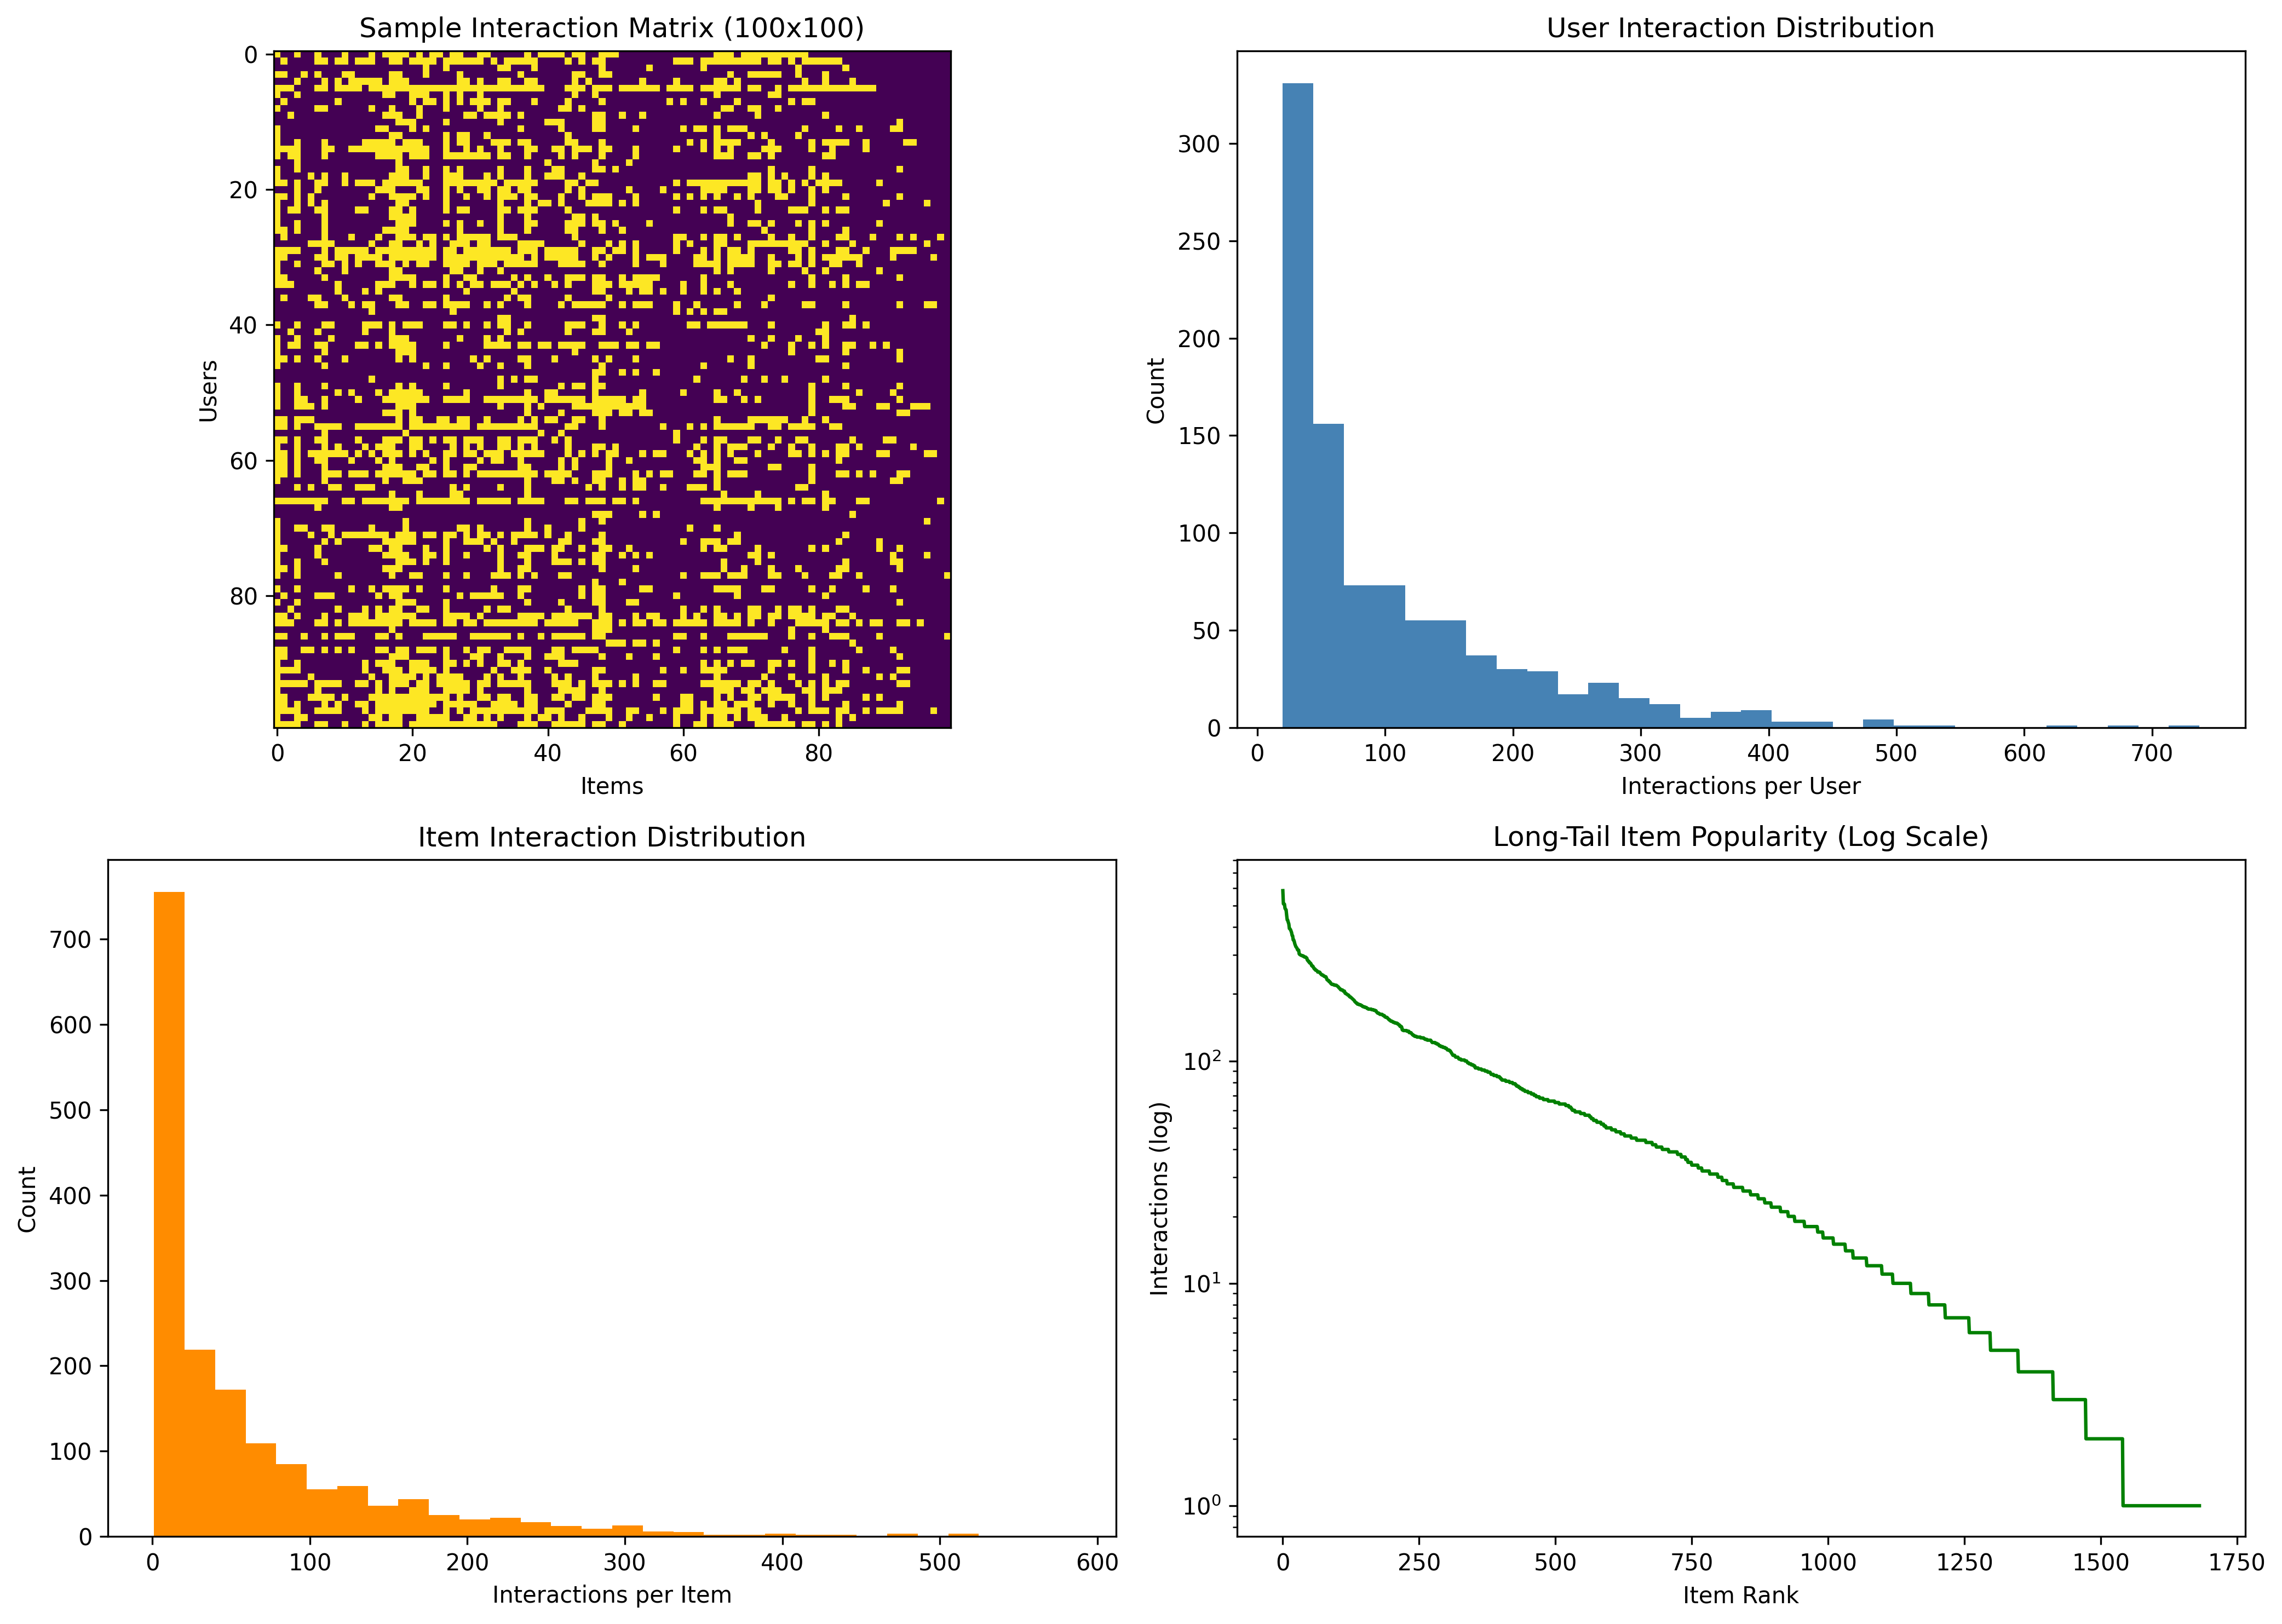
\includegraphics[width=0.68\linewidth]{ml100k_graph.png}

\vspace{0.4cm}

\small
MovieLens 100K exhibits \textbf{93.7\% sparsity} and strong
\textbf{long-tail item popularity}, motivating graph-based learning methods.

\end{frame}

%------------------------------------------------
% Slide 21
% MovieLens-100K — Slide 2 (Statistics + PCA)

\begin{frame}{MovieLens-100K: Statistics}

\small

\begin{columns}

% Left: Table
\begin{column}{0.45\textwidth}
\begin{table}
\centering
\begin{tabular}{l l}
\hline
\textbf{Property} & \textbf{Value} \\
\hline
Users & 943 \\
Items & 1,682 \\
Interactions & 100,000 \\
Density & 0.063 \\
Sparsity & 93.7\% \\
\hline
\end{tabular}
\end{table}
\end{column}

% Right: PCA image
\begin{column}{0.55\textwidth}
\centering
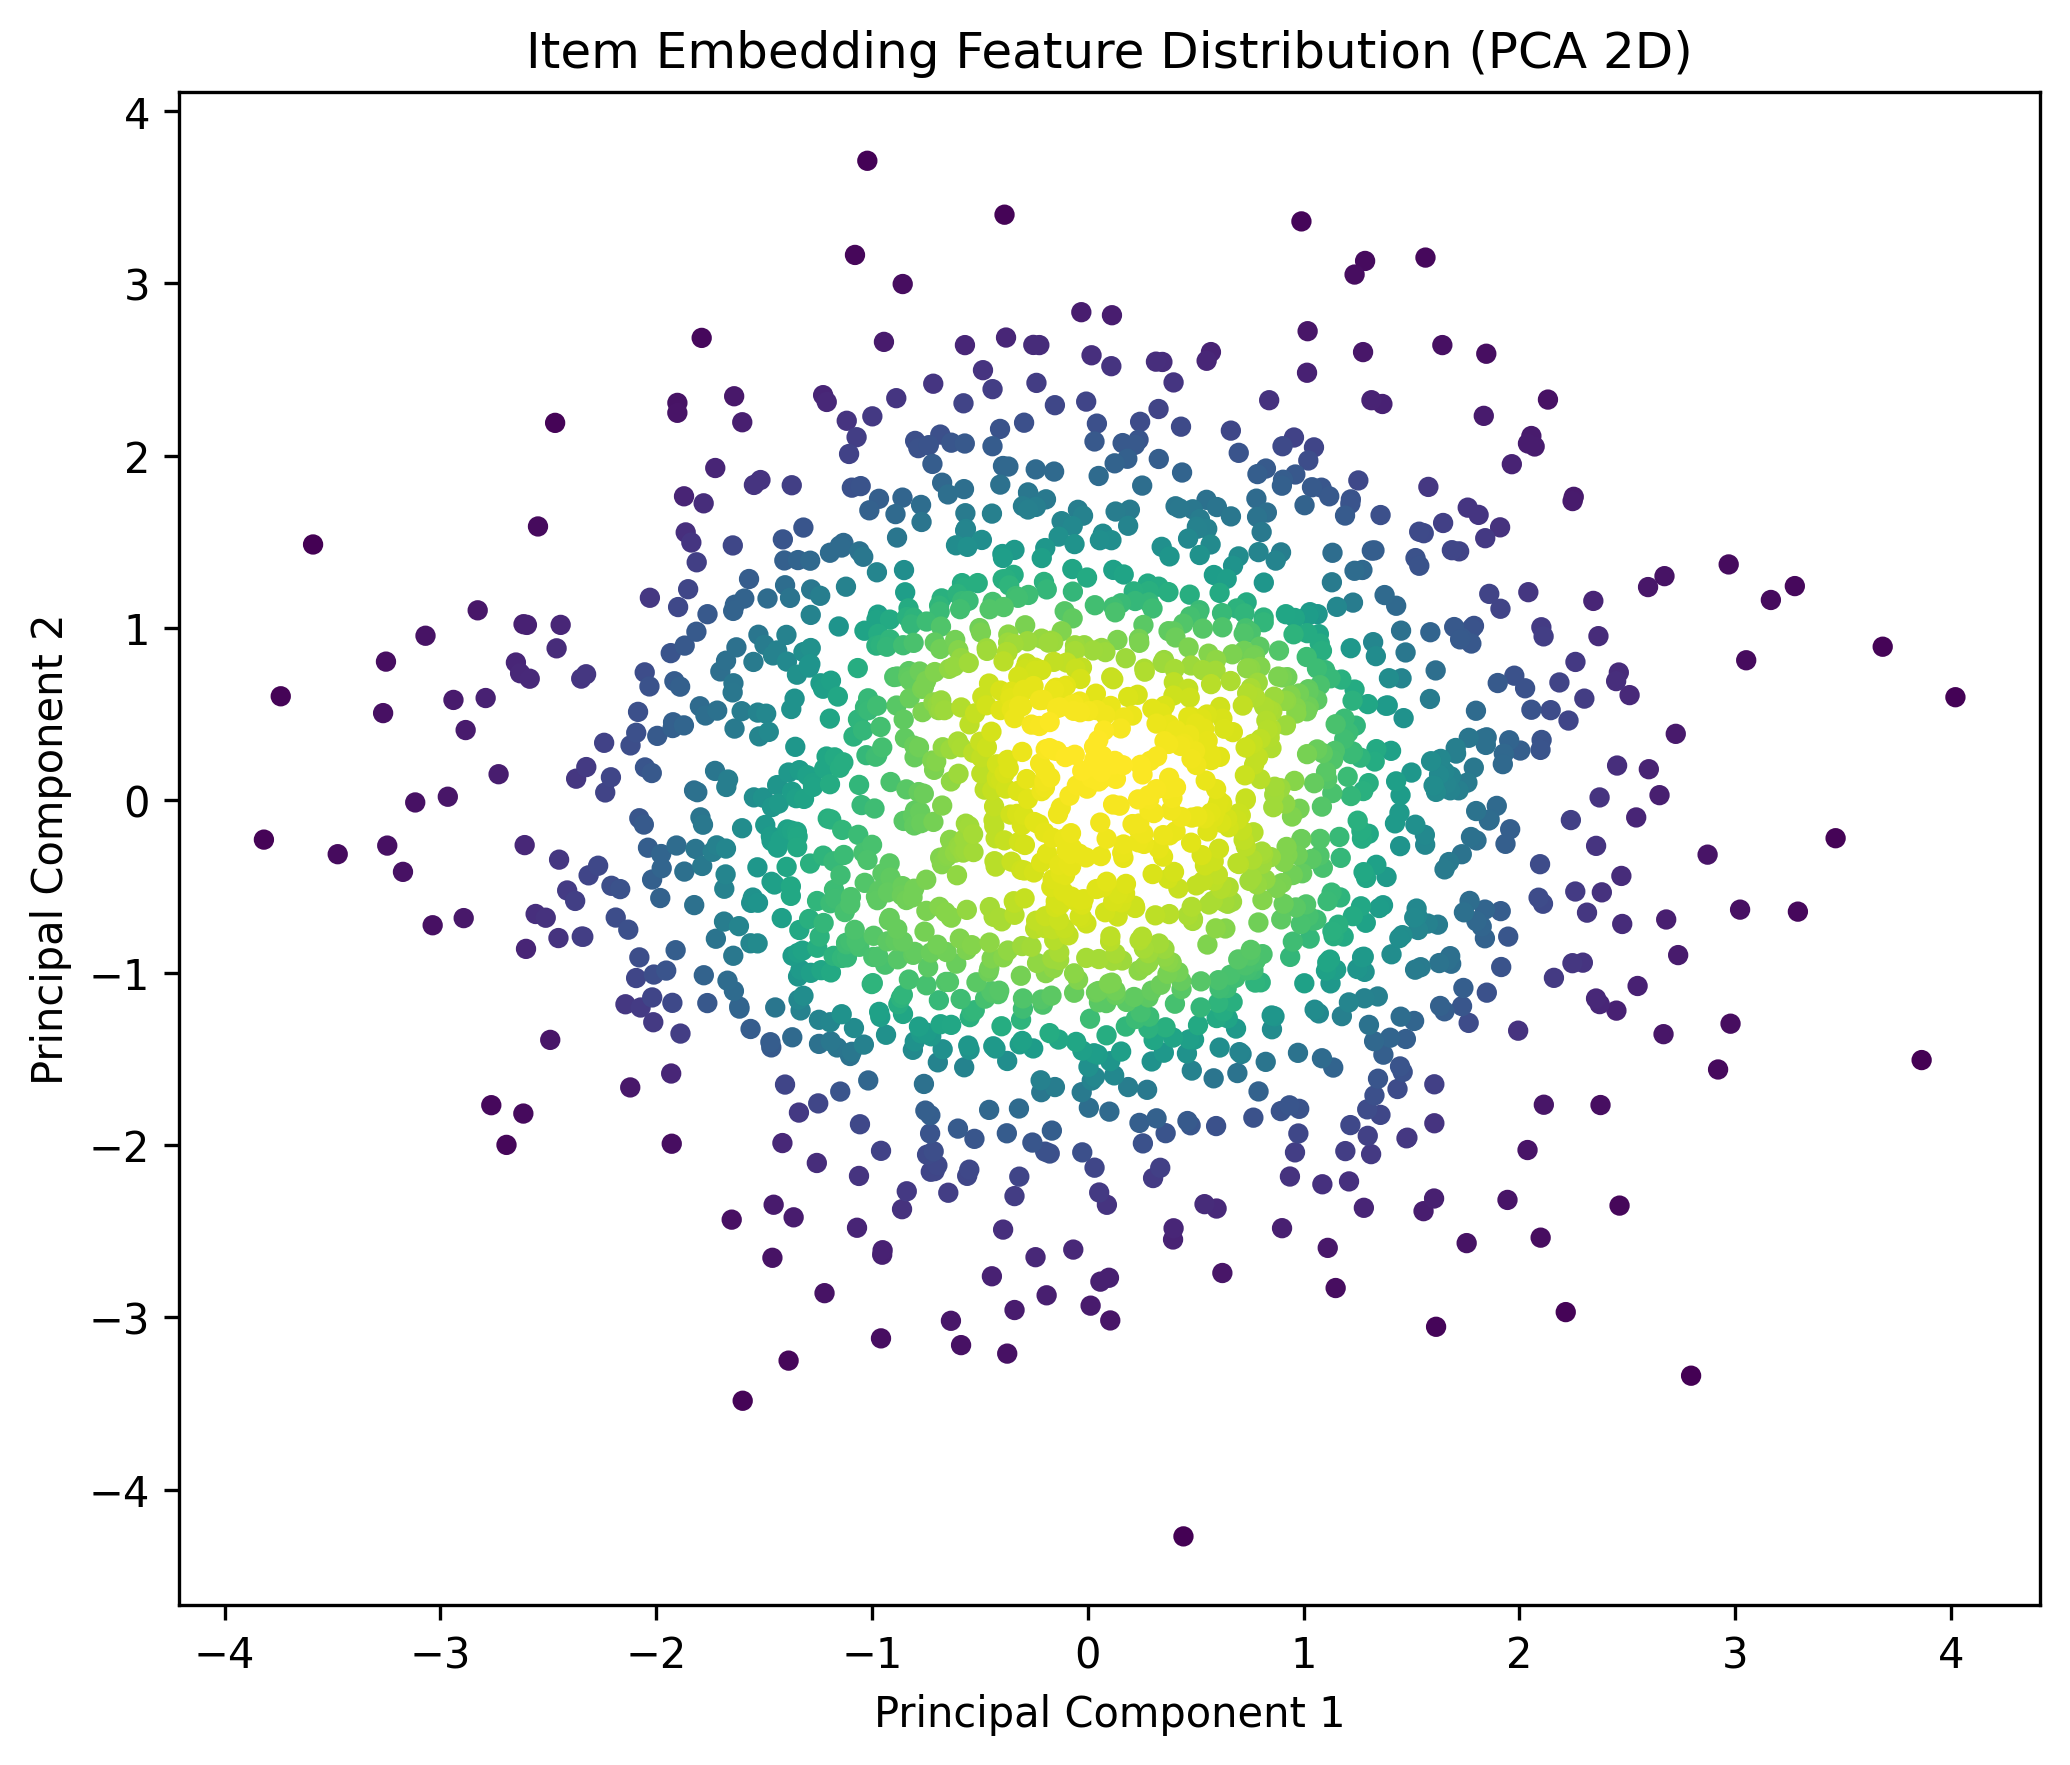
\includegraphics[width=\linewidth]{ml100k_pca.png}
\end{column}

\end{columns}

\vspace{0.3cm}

The PCA projection shows clustering behavior in latent space,
reflecting structural similarity learned by the model.

\end{frame}


%================================================
% Slide 22
% Steam-200K — Slide 1 (Graph + Text)

\begin{frame}{Steam-200K Dataset (Analyzed by Saumya Suman)}

\centering
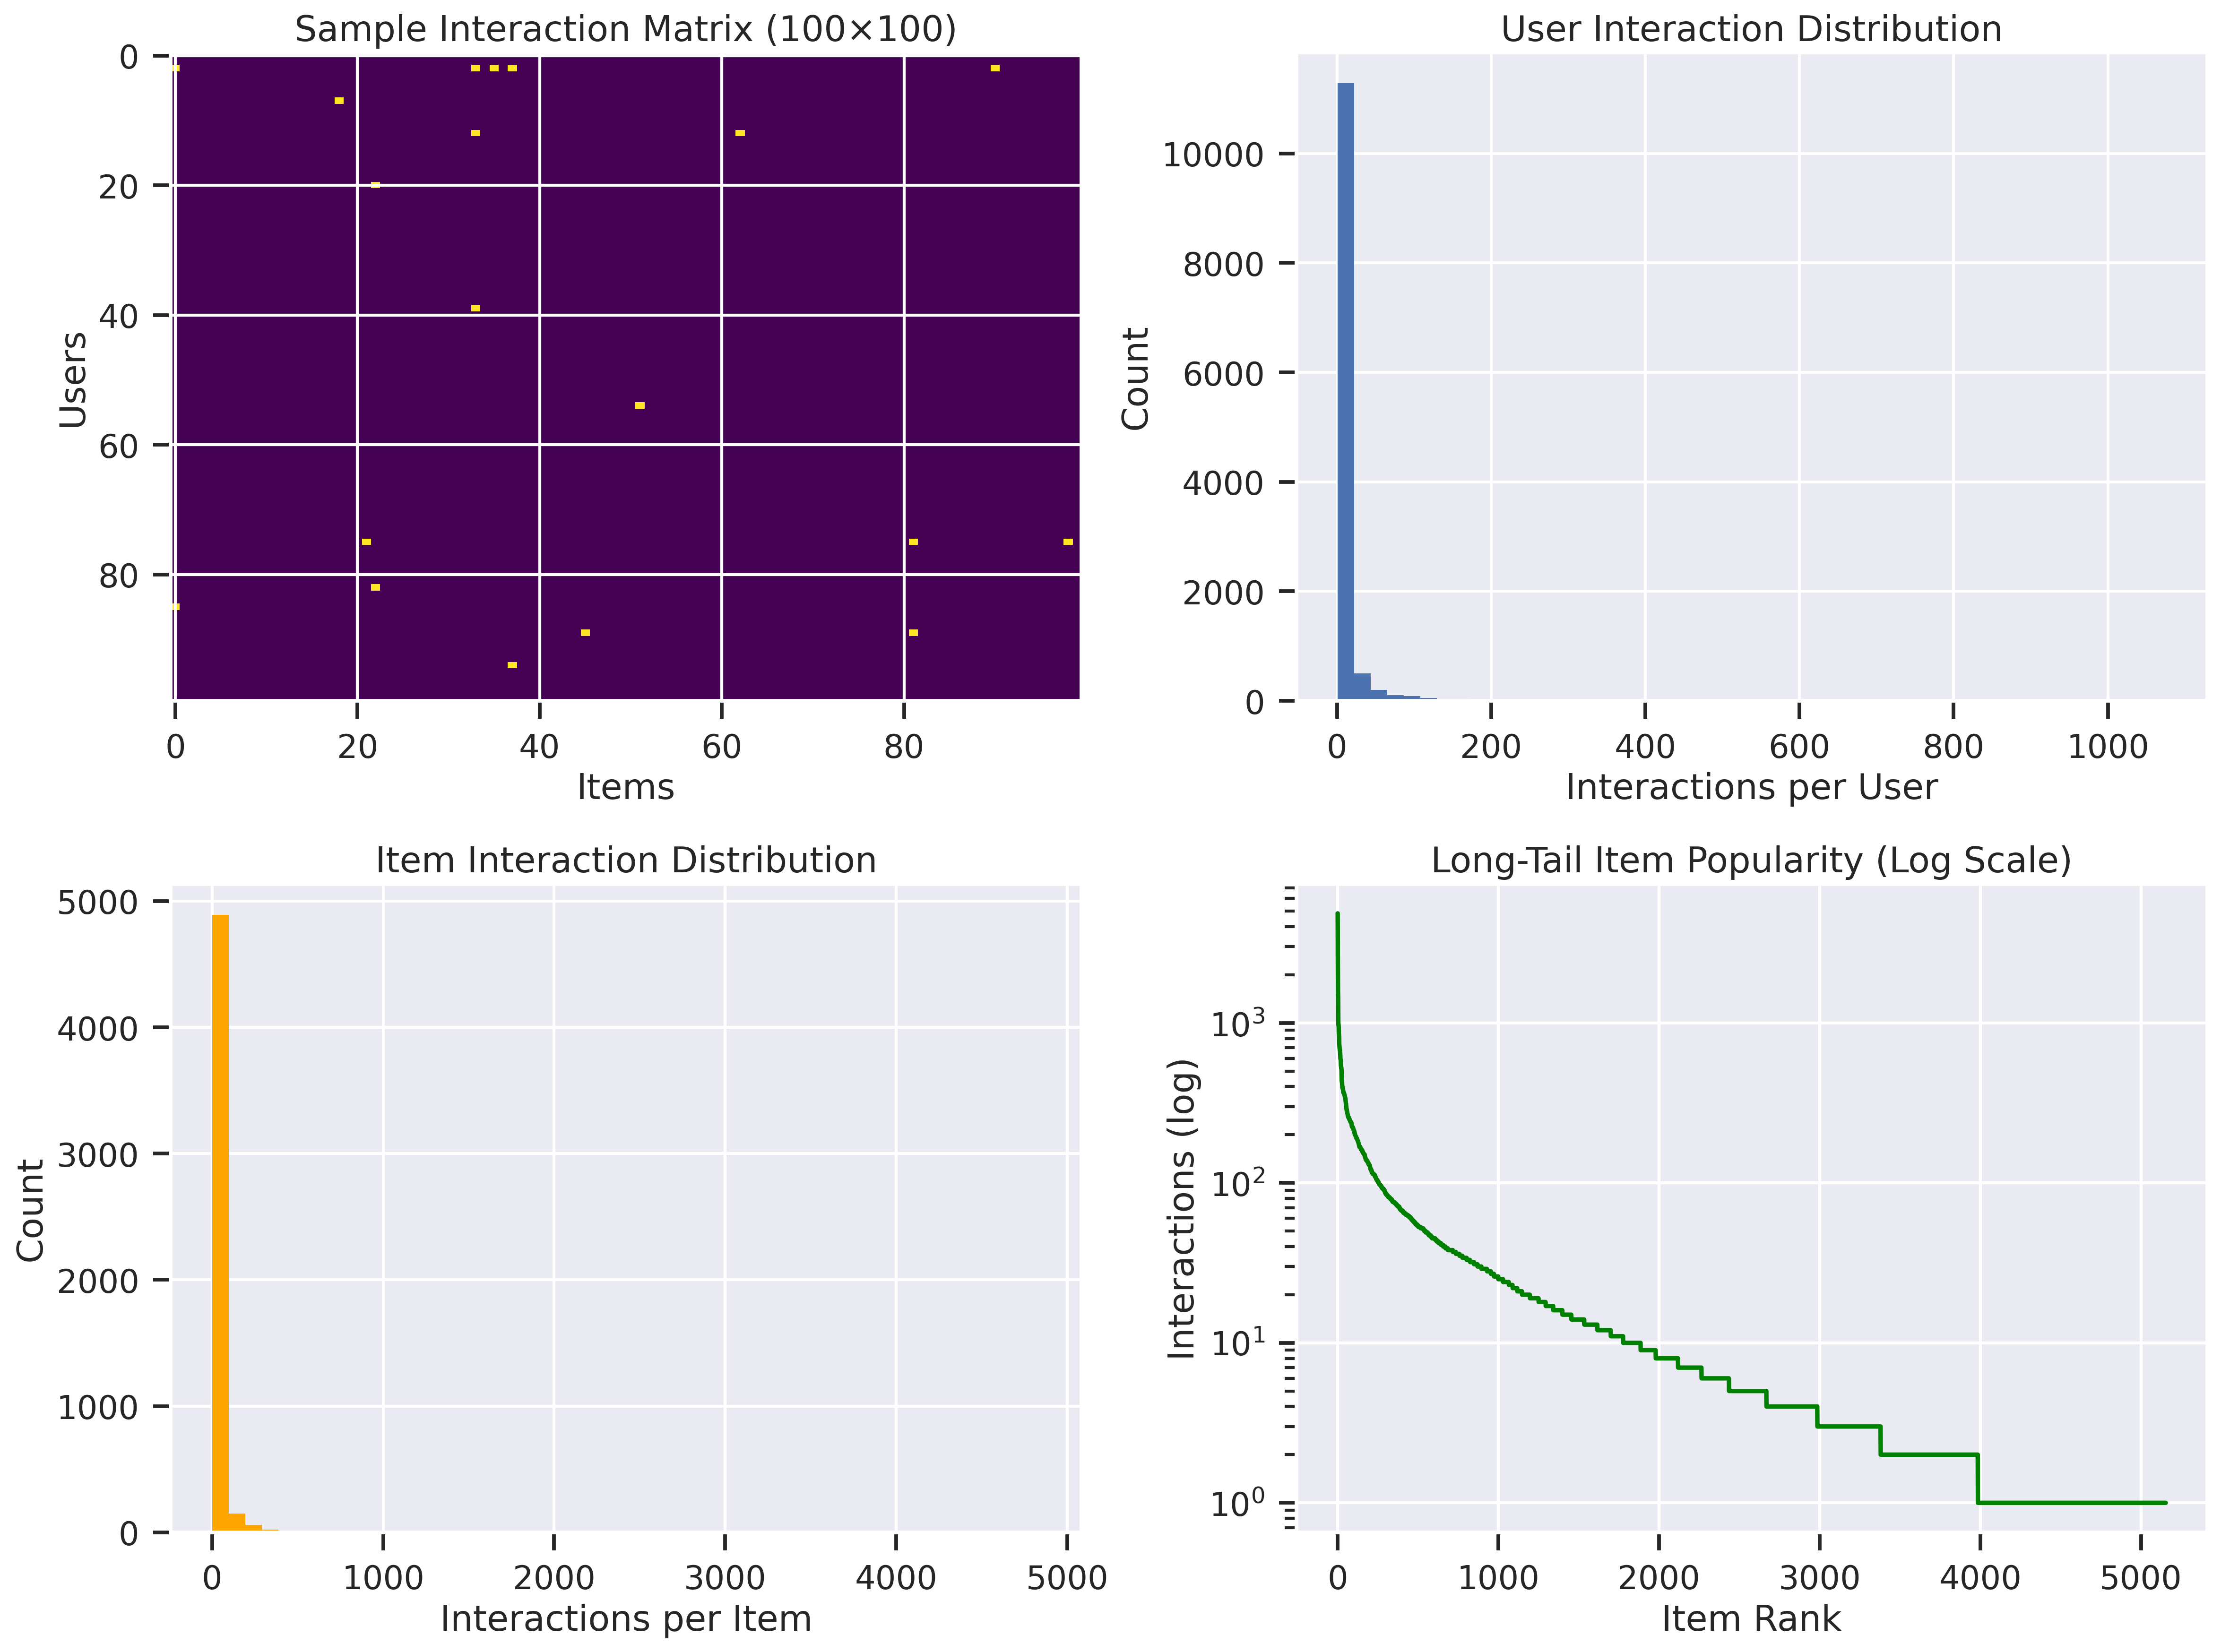
\includegraphics[width=0.66\linewidth]{steam_graph.png}

\vspace{0.4cm}

\small
Steam-200K is an \textbf{extremely sparse dataset} with 
\textbf{99.8\% sparsity}, posing significant challenges 
for collaborative filtering.

\end{frame}

%------------------------------------------------
% Slide 23
% Steam-200K — Slide 2 (Statistics + PCA)

\begin{frame}{Steam-200K: Statistics}

\small

\begin{columns}

% Left: Table
\begin{column}{0.45\textwidth}
\begin{table}
\centering
\begin{tabular}{l l}
\hline
\textbf{Property} & \textbf{Value} \\
\hline
Users & $\sim$3,753 \\
Items & 5,134 \\
Interactions & 114,713 \\
Density & 0.0020 \\
Sparsity & 99.8\% \\
\hline
\end{tabular}
\end{table}
\end{column}

% Right: PCA image
\begin{column}{0.55\textwidth}
\centering
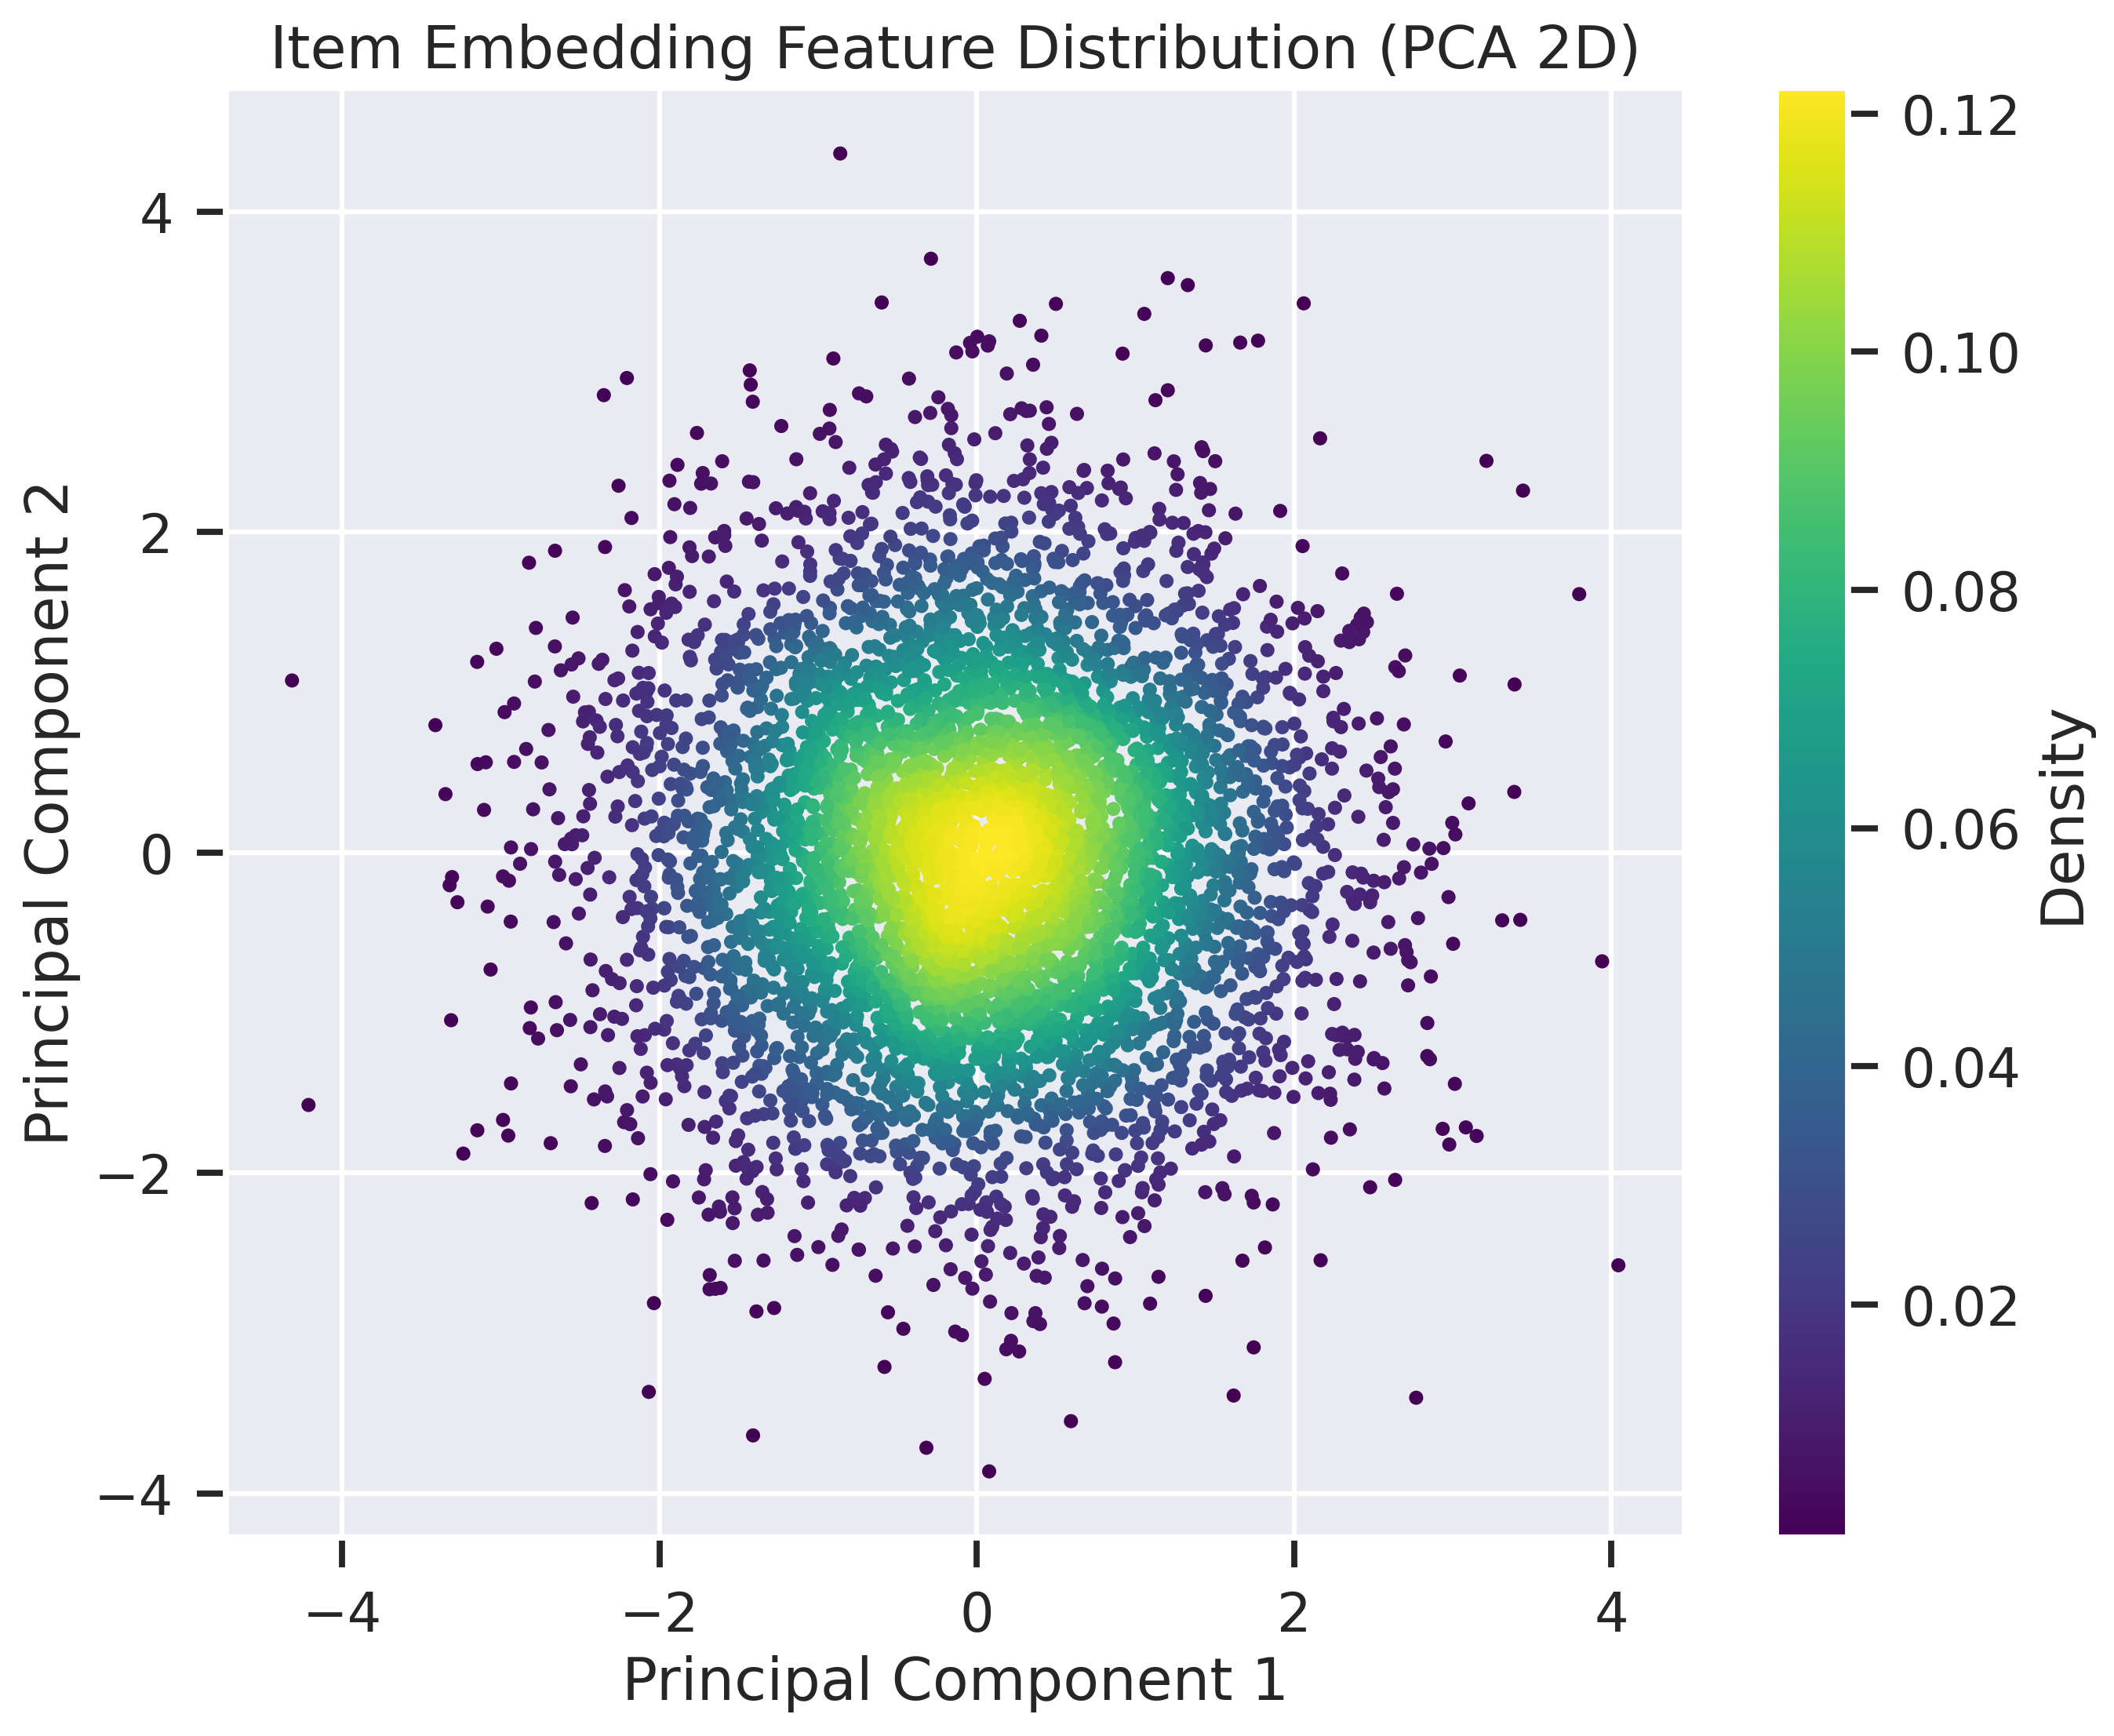
\includegraphics[width=\linewidth]{steam_pca.png}
\end{column}

\end{columns}

\vspace{0.3cm}

The PCA projection reveals emerging latent structure 
despite extreme sparsity.

\end{frame}




%================================================
% Slide 24
% FilmTrust — Slide 1 (Graph + Text)

\begin{frame}{FilmTrust Dataset (Analyzed by Mithil Patidar)}

\centering
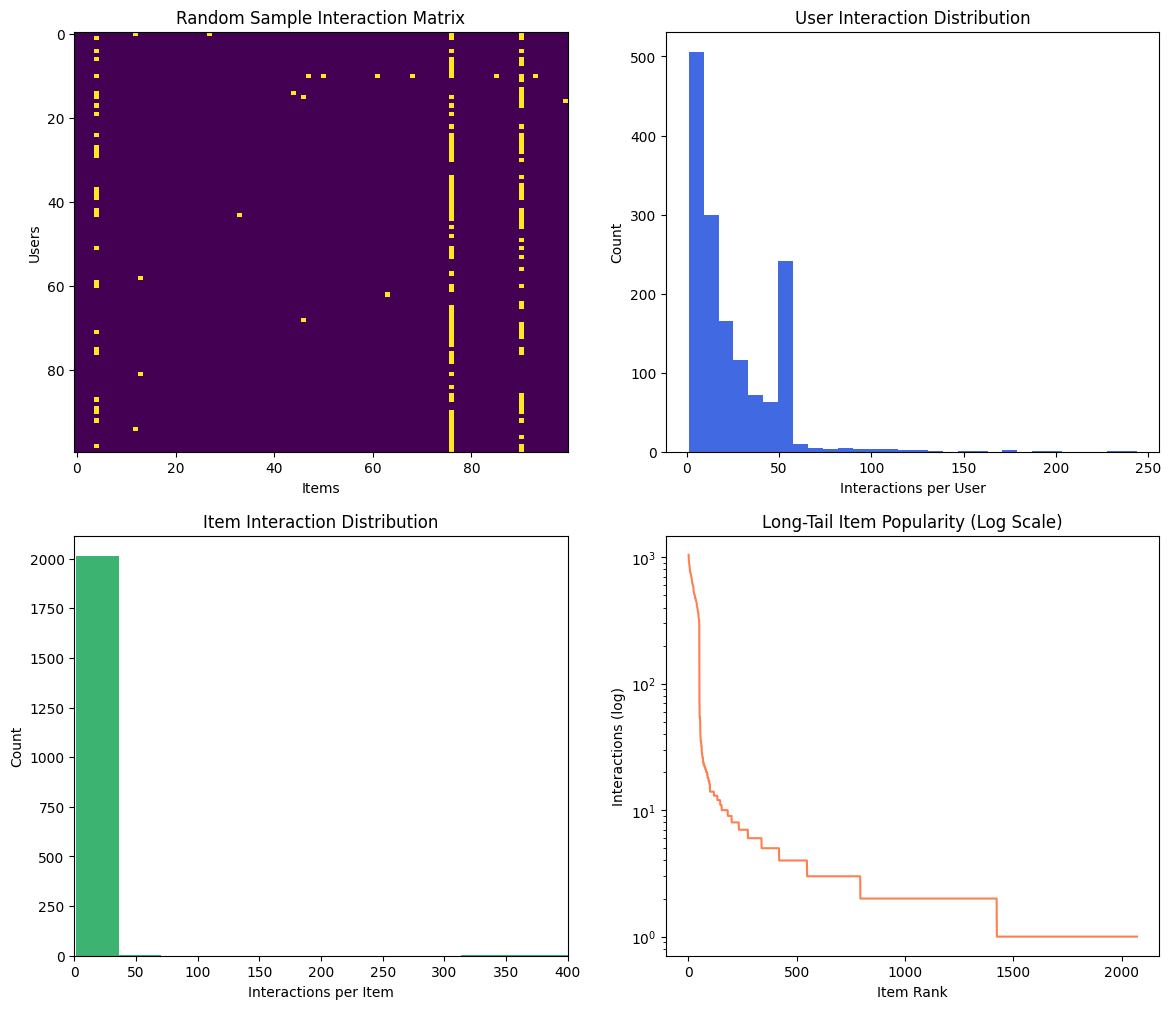
\includegraphics[width=0.58\linewidth]{filmtrust_graph.png}

\vspace{0.4cm}

\small
FilmTrust is a \textbf{sparse trust-aware dataset}, 
making it suitable for evaluating personalization 
under limited user feedback.

\end{frame}

%------------------------------------------------
% Slide 25
% FilmTrust — Slide 2 (Statistics + PCA)

\begin{frame}{FilmTrust: Statistics}

\small

\begin{columns}

% Left: Table
\begin{column}{0.45\textwidth}
\begin{table}
\centering
\begin{tabular}{l l}
\hline
\textbf{Property} & \textbf{Value} \\
\hline
Users & 1,110 \\
Items & 1,775 \\
Interactions & 20,453 \\
Density & 0.0113 \\
Sparsity & 98.8\% \\
\hline
\end{tabular}
\end{table}
\end{column}

% Right: PCA image
\begin{column}{0.55\textwidth}
\centering
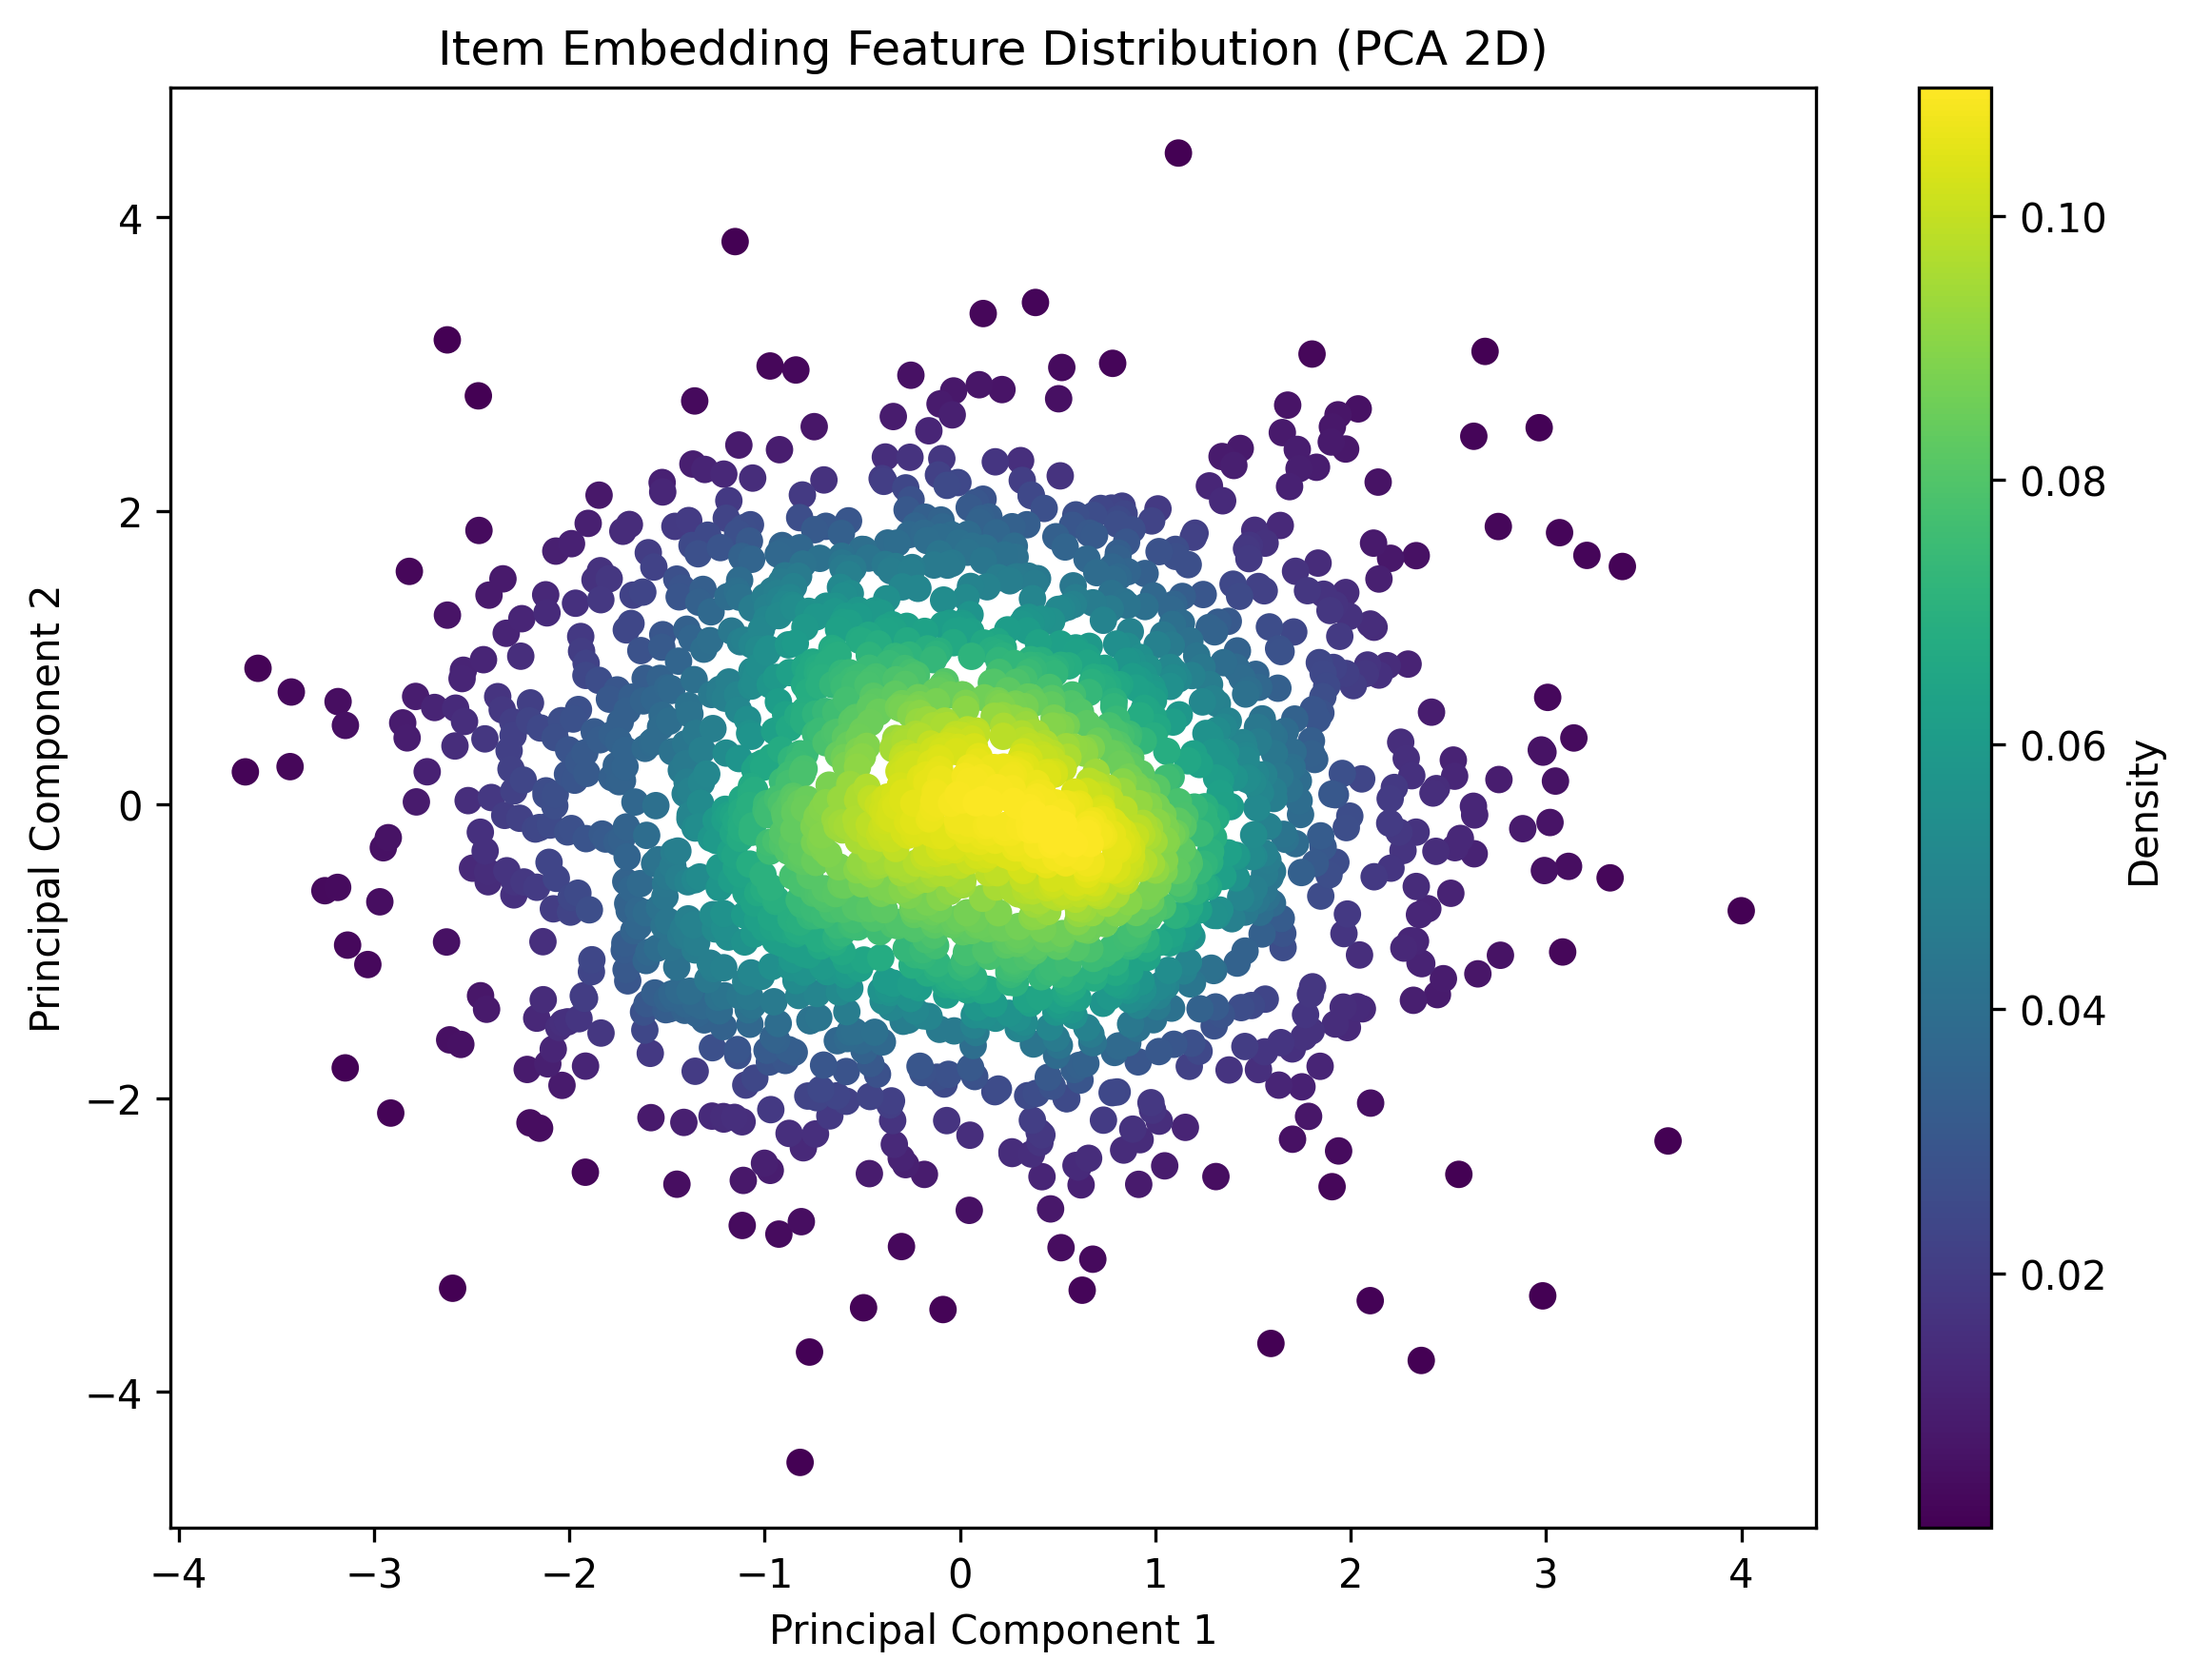
\includegraphics[width=\linewidth]{filmtrust_pca.png}
\end{column}

\end{columns}

\vspace{0.3cm}

The PCA projection shows latent structure 
supporting personalized aggregation.

\end{frame}




%-----------------------------------------------------
\section{Baseline Models}

% Slide 26
\begin{frame}{Baseline models}
\small
\begin{itemize}
  \item \textbf{LightGCN} (He et al., SIGIR 2020)
  {\color{blue}\hyperlink{ref:lightgcn}{\textit{[1]}}}:
  Centralized GNN-based recommender that simplifies GCNs by removing
  feature transformation and nonlinear activation, using neighborhood
  aggregation for collaborative filtering.

  \item \textbf{FedAvg} (McMahan et al., 2017)
  {\color{blue}\hyperlink{ref:fedavg}{\textit{[2]}}}:
  Standard federated learning algorithm that aggregates client models
  via weighted averaging, assuming IID data distribution across clients.

  \item \textbf{FedMF} (Chai et al., 2021)
  {\color{blue}\hyperlink{ref:fedmf}{\textit{[3]}}}:
  Federated matrix factorization framework that jointly learns item
  embeddings while keeping user embeddings local, using homomorphic
  encryption to protect gradient privacy.
\end{itemize}
\end{frame}


% Slide 27
\begin{frame}{Baseline models (cont.)}
\small
\begin{itemize}

  \item \textbf{FedGNN} (Wu et al.)
  {\color{blue}\hyperlink{ref:fedgnn}{\textit{[4]}}}:
  Privacy-preserving federated recommendation method that applies GNNs
  on decentralized user–item graphs and introduces pseudo-interaction
  sampling to mitigate privacy leakage.

  \item \textbf{PerFedRec} (Luo et al., 2022)
  {\color{blue}\hyperlink{ref:perfedrec}{\textit{[5]}}}:
  Personalized federated GNN-based recommender that clusters users and
  adapts models locally to alleviate performance degradation caused by
  non-IID data.

  \item \textbf{FPFR} (Zhang et al.)
  {\color{blue}\hyperlink{ref:fpfr}{\textit{[6]}}}:
  Fair and personalized federated recommendation framework that
  introduces attention-based personalization and fairness-aware
  objectives during federated aggregation.

\end{itemize}
\end{frame}


%-----------------------------------------------------
% Slide 28
\begin{frame}{Evaluation metrics}
  \begin{itemize}
    \item \textbf{Hit Rate @ 10 (HR@10)}: fraction of users for whom the test item appears in top-10 recommendations.
    \item \textbf{NDCG(Normalized Discounted Cumulative Gain) @ 10}: normalized discounted cumulative gain; accounts for ranking position (higher weight to hits at top positions).
    \item \textbf{Evaluation protocol} : leave-one-out test (last interaction for test), sample 100 negatives per user and combining test items and sample negatives.
  \end{itemize}
\end{frame}

\section{Summary}

% Slide 29
\begin{frame}{Performance summary}
\scriptsize

\resizebox{\textwidth}{!}{
\begin{tabular}{l l c c c c c c c c}
\hline
\textbf{Dataset} & \textbf{Metric} & \textbf{Central} & \textbf{FedAvg} & \textbf{FedMF} & \textbf{FedGNN} & \textbf{PerFedRec} & \textbf{FPFR} & \textbf{FedPCL} & \textbf{Improv} \\
\hline

\multirow{2}{*}{ML-1M}
& HR@10   & 64.53 & 44.70 & 56.30 & 58.37 & 61.31 & 61.84 & \textbf{62.86} & 1.65\% \\
& NDCG@10 & 46.78 & 24.90 & 31.30 & 39.84 & 42.83 & 43.62 & \textbf{44.12} & 1.15\% \\
\hline

\multirow{2}{*}{ML-100K}
& HR@10   & 64.31 & 42.70 & 58.34 & 60.30 & 61.87 & 62.59 & \textbf{63.81} & 1.95\% \\
& NDCG@10 & 45.57 & 23.87 & 32.82 & 43.03 & 43.51 & 44.65 & \textbf{45.03} & 0.85\% \\
\hline

\multirow{2}{*}{Steam}
& HR@10   & 80.16 & 71.21 & 73.82 & 75.33 & 76.61 & 78.43 & \textbf{80.36} & 2.46\% \\
& NDCG@10 & 66.03 & 50.22 & 54.09 & 62.09 & 62.63 & 64.76 & \textbf{65.55} & 1.22\% \\
\hline

\multirow{2}{*}{FilmTrust}
& HR@10   & 21.85 & 10.81 & 11.85 & 15.58 & 15.12 & 15.66 & \textbf{16.81} & 7.34\% \\
& NDCG@10 & 10.53 & 4.83  & 5.82  & 8.17  & 8.01  & 8.04  & \textbf{8.61}  & 5.39\% \\
\hline

\multirow{2}{*}{Amazon-Elec}
& HR@10   & 38.83 & 26.53 & 28.22 & 30.40 & 32.64 & 32.76 & \textbf{34.04} & 3.91\% \\
& NDCG@10 & 26.74 & 14.53 & 18.55 & 18.97 & 21.39 & 21.98 & \textbf{22.93} & 4.32\% \\
\hline

\end{tabular}
}

\vspace{0.35cm}

FedPCL consistently outperforms other federated baselines across
all five datasets reported in the paper.

\vspace{0.2cm}

\textbf{In all five datasets, average improvement in HR@10: 3.46\%,
and in NDCG@10: 2.59\%.}

\end{frame}


%-----------------------------------------------------
%-----------------------------------------------------
% Slide 30
\begin{frame}{Parameter Sensitivity \& Experimental Settings}
\small
\begin{itemize}

\item \textbf{Temperature $\tau$ (Contrastive Learning):}
      Tested in $[0.125, 0.225]$; 
      Best performance at $\tau \approx 0.175$--$0.20$.
      (Default setting: $\tau = 0.3$)

\item \textbf{Contrast Weight $\lambda$ (User vs Item CL):}
      Tested in $[0.2, 1.8]$; 
      Optimal near $\lambda = 1$.
      (Default setting: $\lambda = 1$)

\item \textbf{Number of Clusters $K$ (Personalization):}
      Tested in $\{0,5,10,15,20\}$; 
      Default $K = 5$.
      Removing clustering ($K=0$) degrades performance.

\item \textbf{Other Key Hyperparameters:}
      \begin{itemize}
          \item Learning rate $\eta = 0.1$
          \item Embedding dimension $d = 64$
          \item L2 Regularization $= 1e^{-6}$
          \item Personalization weights $\mu_1 = \mu_2 = 0.5$
          \item Communication rounds $T = 400$
          \item Clients per round $= 128$
      \end{itemize}

\end{itemize}

\end{frame}


%-----------------------------------------------------
% Slide 31
\begin{frame}{Future Work / Research Directions}
\small
\begin{itemize}

\item \textbf{Advanced Clustering Strategies:}  
Replace fixed K-means with more adaptive methods such as 
Advanced/Improved K-means, Spectral Clustering, or Graph-based clustering 
to better capture user similarity in non-IID federated settings.

\item \textbf{Dynamic \& Online Cluster Updating:}  
Design time-aware or incremental clustering mechanisms 
to handle evolving user preferences and continuously update 
cluster assignments during training.

\item \textbf{Scalable \& Robust Federated Optimization:}  
Incorporate communication-efficient aggregation, adaptive weighting of cluster/global models, 
and stronger privacy guarantees for large-scale real-world deployment.

\end{itemize}

\end{frame}

%-----------------------------------------------------
% Slide 32
\begin{frame}{Conclusion}
  \begin{itemize}
    \item FedPCL presents an effective framework that integrates structural contrastive learning with personalized federated aggregation.
    
    \item The proposed combination addresses two major challenges in federated recommendation systems:
    \begin{itemize}
        \item Data sparsity
        \item Non-IID data heterogeneity
    \end{itemize}
    
    \item We successfully reproduced and analyzed the method on three benchmark datasets:
    \textbf{ML-100K, Steam-200K, and FilmTrust}, validating the core contributions of the paper.
  \end{itemize}
\end{frame}


%-----------------------------------------------------
% Slide 33
\begin{frame}{Progress}
\begin{itemize}

  \item We have completed dataset preprocessing and analyzed key statistics such as sparsity, density, and interaction distribution.

  \item We are currently working on the core components of the FedPCL framework, including GNN modeling, contrastive loss, and federated aggregation setup.

  \item We are currently working on reproducing the experimental results reported in the paper and tuning hyperparameters to match the published performance.

\end{itemize}
\end{frame}



%------------------------------------------------
% Slide 34
\begin{frame}{References (1/2)}
\small

\begin{enumerate}

  \item \hypertarget{ref:lightgcn}{}
  X. He, K. Deng, X. Wang, Y. Li, Y. Zhang, and M. Wang,
  \emph{LightGCN: Simplifying and Powering Graph Convolution Network
  for Recommendation},
  Proceedings of SIGIR, 2020.

  \item \hypertarget{ref:fedavg}{}
  H. B. McMahan, E. Moore, D. Ramage, S. Hampson, and B. A. y Arcas,
  \emph{Communication-Efficient Learning of Deep Networks from
  Decentralized Data},
  Proceedings of AISTATS, 2017.

  \item \hypertarget{ref:fedmf}{}
  D. Chai, L. Wang, K. Chen, and Q. Yang,
  \emph{Secure Federated Matrix Factorization},
  IEEE Transactions on Knowledge and Data Engineering, 2021.

\end{enumerate}

\end{frame}

%------------------------------------------------
% Slide 35
\begin{frame}{References (2/2)}
\small

\begin{enumerate}
  \setcounter{enumi}{3} % starts numbering from 4

  \item \hypertarget{ref:fedgnn}{}
  C. Wu, F. Wu, T. Qi, and Y. Huang,
  \emph{Federated Graph Neural Networks for Recommendation},
  2021.

  \item \hypertarget{ref:perfedrec}{}
  X. Luo, Y. Wang, L. Li, J. Li, and Z. Ren,
  \emph{PerFedRec: Personalized Federated Recommendation},
  Proceedings of CIKM, 2022.

  \item \hypertarget{ref:fpfr}{}
  Z. Zhang, Y. Wu, J. Fan, and Q. Yang,
  \emph{FPFR: Fair and Personalized Federated Recommendation},
  2023.

  \item \hypertarget{ref:fedpcl}{}
  \textbf{S. Wang, Y. Zhou, X. Fan, J. Li, Z. Lei, and M. Gong,} \\
  \textbf{\emph{Personalized Federated Contrastive Learning for Recommendation},IEEE Transactions on Computational Social Systems, 2025.}

\end{enumerate}

\end{frame}


%------------------------------------------------
% Slide 36
\begin{frame}{Thank You}
\centering
\Huge Thank You!! \\
\vspace{1cm}
\end{frame}

\end{document}
